% =====================================================================
%  Chapitre 2 -- L'operation de convolution
%  Partie b : padding, stride, dimensions, champ recepteur
% =====================================================================

\begin{frame}{Le problème des bords}
\begin{columns}[t]
\begin{column}{0.52\textwidth}
\begin{itemize}
  \item Un noyau $3 \times 3$ posé sur le coin d'une image $5 \times 5$
  déborde : il lui faut des pixels qui n'existent pas.
  \item Deux choix seulement :
  \begin{itemize}
    \item \textbf{valid} : on ne pose le noyau que là où il tient
    entièrement --- l'image rétrécit ;
    \item \textbf{same} : on ajoute une bordure de zéros
    (\textbf{padding}) --- l'image garde sa taille.
  \end{itemize}
\end{itemize}
\begin{kbox}[Padding = 1 pour un noyau $3 \times 3$]
En général $P = (K-1)/2$, ce qui donne $P=1$ pour $K=3$ et $P=2$ pour $K=5$.
\end{kbox}
\end{column}
\begin{column}{0.44\textwidth}
\centering
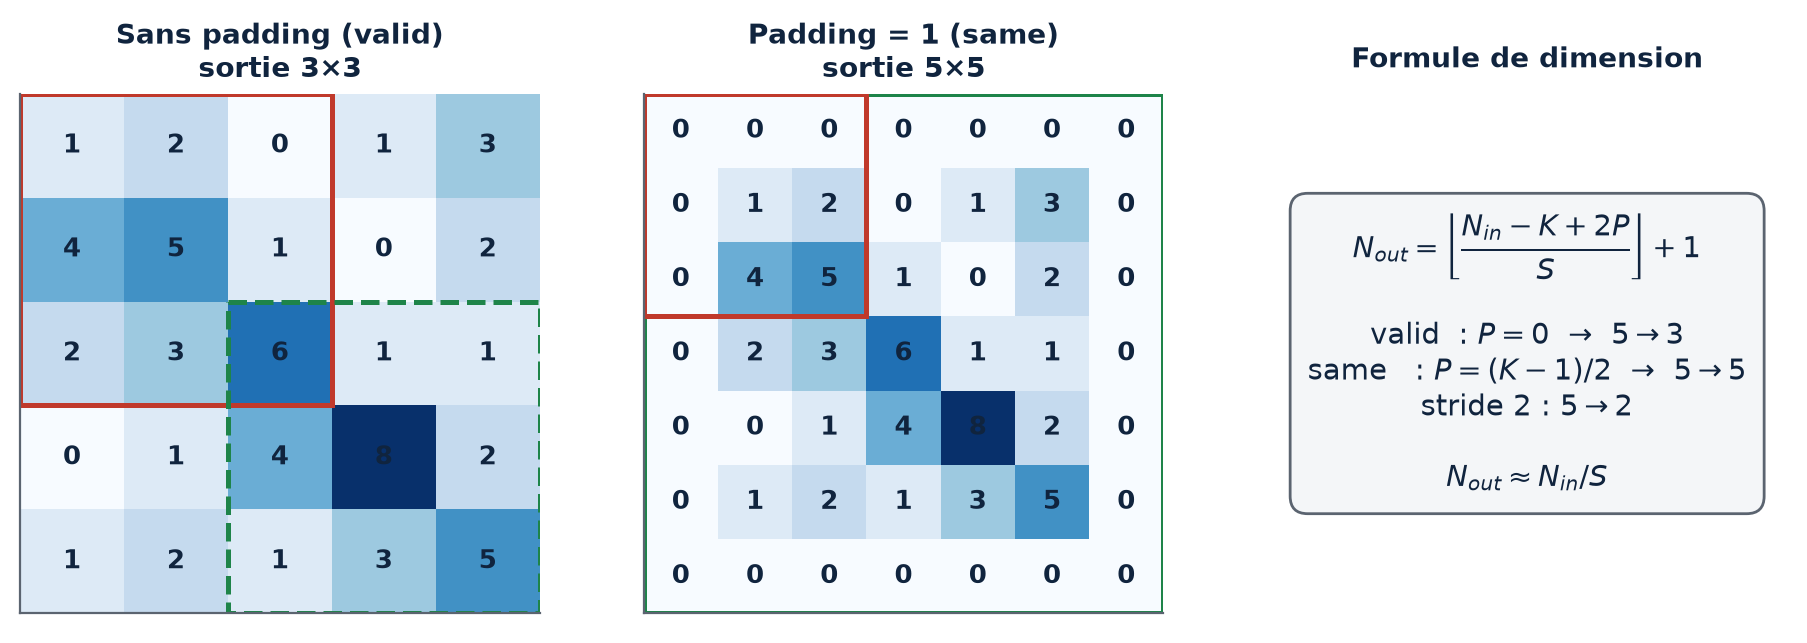
\includegraphics[width=\textwidth]{g05_padding.png}
\end{column}
\end{columns}
\end{frame}

\begin{frame}{La formule de dimension --- la plus importante du cours}
\begin{columns}[t]
\begin{column}{0.52\textwidth}
\begin{center}
\large
$N_{out} = \left\lfloor \dfrac{N_{in} - K + 2P}{S} \right\rfloor + 1$
\end{center}
\vspace{2mm}
\begin{itemize}
  \item $N_{in}$ : côté de l'entrée \quad $K$ : côté du noyau
  \item $P$ : padding \quad $S$ : stride
  \item Elle s'applique \textbf{indépendamment} en largeur et en hauteur.
\end{itemize}
\begin{wbox}[Le piège classique]
Oublier le $+1$. Sans lui, une entrée de taille égale au noyau donnerait
$0$ --- alors qu'elle donne $1$.
\end{wbox}
\end{column}
\begin{column}{0.44\textwidth}
\begin{ebox}[Vérification sur nos exemples]
\begin{center}
\begin{tabular}{@{}lccc@{}}
\toprule
$N_{in}$ & $K$ & $P$ & $N_{out}$ \\
\midrule
5 & 3 & 0 & 3 \\
5 & 3 & 1 & 5 \\
5 & 3 & 0 (S=2) & 2 \\
28 & 3 & 0 & 26 \\
32 & 5 & 0 & 28 \\
\bottomrule
\end{tabular}
\end{center}
\end{ebox}
\end{column}
\end{columns}
\end{frame}

\begin{frame}{Le stride : balayer plus vite, voir plus loin}
\begin{columns}[t]
\begin{column}{0.48\textwidth}
\centering
\end{column}
\begin{column}{0.48\textwidth}
\begin{itemize}
  \item \textbf{stride 1} : le noyau avance d'un pixel --- sortie
  $5 \times 5 \to 3 \times 3$ (valid).
  \item \textbf{stride 2} : il avance de deux pixels --- sortie
  $5 \times 5 \to 2 \times 2$.
  \item Le stride \textbf{réduit la résolution} d'un facteur $S$, comme le
  pooling --- mais il apprend des poids, contrairement au pooling.
\end{itemize}
\begin{kbox}[Stride convolutif vs pooling]
Les deux réduisent la taille. Le stride convolutif le fait \emph{en
apprenant} ; le pooling le fait \emph{gratuitement}. Les architectures
modernes remplacent souvent le pooling par un stride 2.
\end{kbox}
\end{column}
\end{columns}
% [fix] figure sortie
\end{frame}

\begin{frame}{Le stride : balayer plus vite, voir plus loin --- la figure}\begin{center}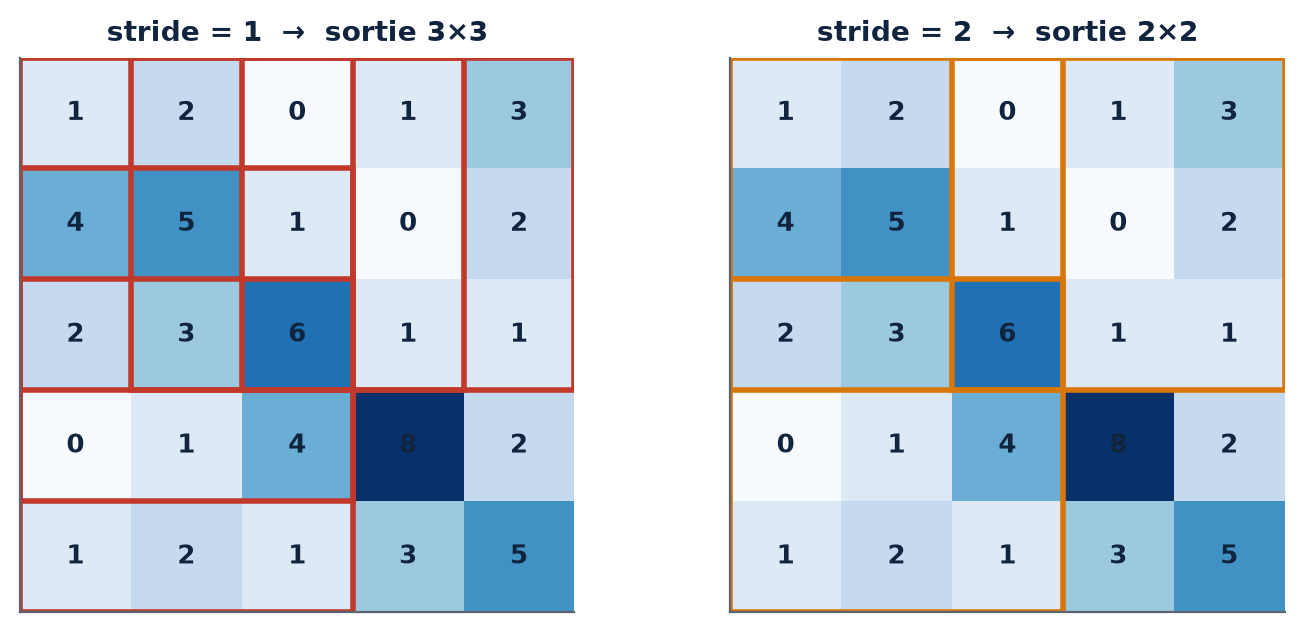
\includegraphics[width=.92\textwidth]{g06_stride.png}\end{center}\end{frame}

\begin{frame}{Lire la carte des dimensions}
\begin{columns}[t]
\begin{column}{0.52\textwidth}
\centering
\end{column}
\begin{column}{0.44\textwidth}
\begin{itemize}
  \item Chaque point de la carte est une combinaison
  ($N_{in}$, $K$) en mode valid.
  \item Plus le noyau est grand, plus la sortie rétrécit : sur une image
  de $28$ pixels, un noyau $11 \times 11$ ne laisse que $18$ pixels.
  \item D'où le rôle du \textbf{padding} : sans lui, dix couches
  convolutives consécutives videraient l'image.
\end{itemize}
\begin{solbox}[Repère MNIST]
$28 \times 28$ avec un noyau $3 \times 3$ en valid donne $26 \times 26$ :
on perd 2 pixels par couche.
\end{solbox}
\end{column}
\end{columns}
% [fix] figure sortie
\end{frame}

\begin{frame}{Lire la carte des dimensions --- la figure}\begin{center}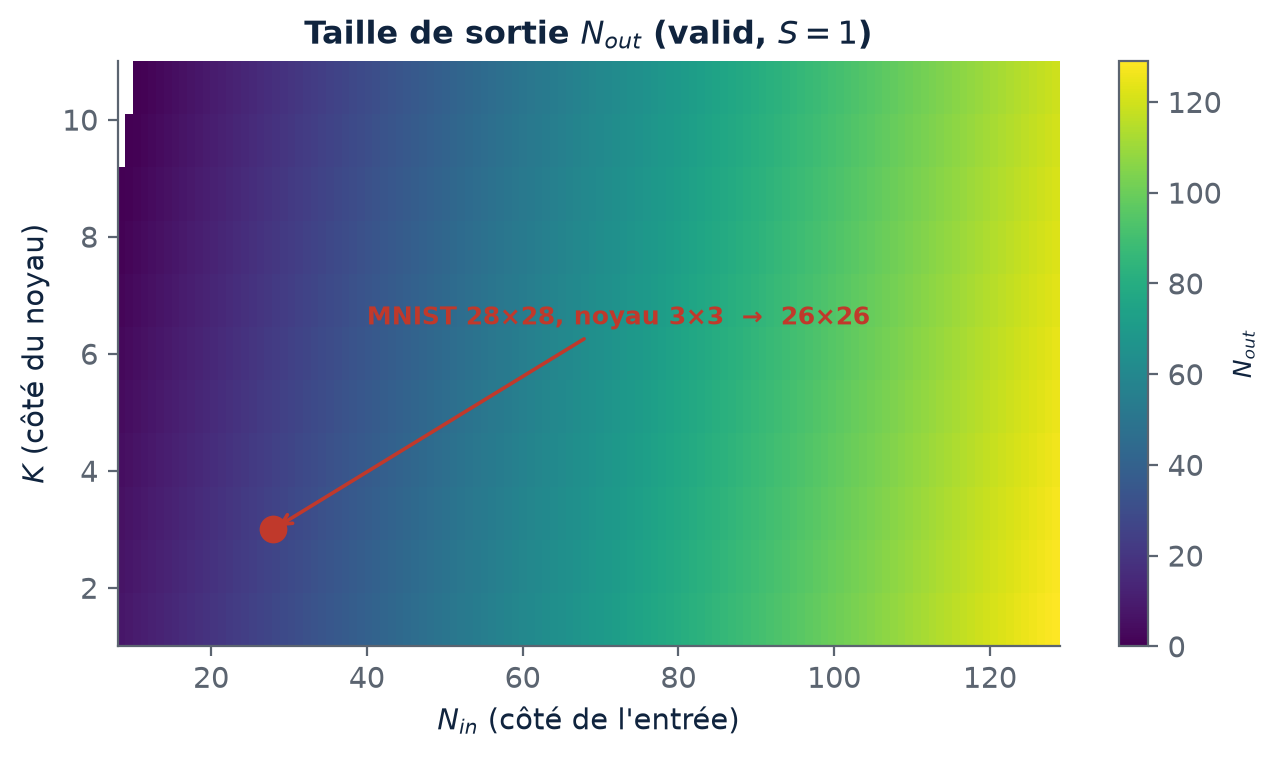
\includegraphics[width=.92\textwidth]{g07_carte_dimensions.png}\end{center}\end{frame}

\begin{frame}[fragile]{Calculer les dimensions, en Python}
\begin{columns}[t]
\begin{column}{0.52\textwidth}
\begin{codebox}[La formule, une seule fois pour toutes]
\begin{lstlisting}
def dim(N_in, K, P=0, S=1):
    return (N_in - K + 2*P)//S + 1

# verifier les exemples du cours
for (N,K,P,S) in [(5,3,0,1), (5,3,1,1),
                  (5,3,0,2), (28,3,0,1)]:
    print(N, K, P, S, "->", dim(N,K,P,S))
\end{lstlisting}
\end{codebox}
\begin{solbox}[Sortie attendue]
\begin{verbatim}
5 3 0 1 -> 3
5 3 1 1 -> 5
5 3 0 2 -> 2
28 3 0 1 -> 26
\end{verbatim}
\end{solbox}
\end{column}
\begin{column}{0.44\textwidth}
\begin{wbox}[La même formule pour la profondeur]
La formule s'applique à la \textbf{hauteur} et à la \textbf{largeur}. La
\textbf{profondeur} (nombre de canaux) suit une autre règle : elle devient le
nombre de filtres de la couche.
\end{wbox}
\begin{ebox}[Exemple]
Entrée $28 \times 28 \times 1$, noyau $3 \times 3$, $16$ filtres,
padding 1 :
sortie $28 \times 28 \times 16$.
\end{ebox}
\end{column}
\end{columns}
\end{frame}

\begin{frame}{Le champ récepteur : ce que « voit » un neurone profond}
\begin{columns}[t]
\begin{column}{0.52\textwidth}
\centering
\end{column}
\begin{column}{0.44\textwidth}
\begin{itemize}
  \item Couche 1 : un neurone voit $3 \times 3$ pixels.
  \item Chaque couche supplémentaire ajoute $K - 1 = 2$ pixels de chaque côté.
  \item Après $5$ couches de noyau $3 \times 3$ :
  $1 + 2 \times 5 = 11 \times 11$ pixels.
  \item Après $10$ couches : $21 \times 21$ pixels.
\end{itemize}
\begin{kbox}[Pourquoi empiler ?]
Un réseau profond voit \textbf{large avec de petits noyaux}. C'est toute la
différence entre un noyau $11 \times 11$ isolé et trois couches
$3 \times 3$ : même champ, mais \textbf{non-linéarités} en plus, et
\textbf{moins de poids}.
\end{kbox}
\end{column}
\end{columns}
% [fix] figure sortie
\end{frame}

\begin{frame}{Le champ récepteur : ce que « voit » un neurone profond --- la figure}\begin{center}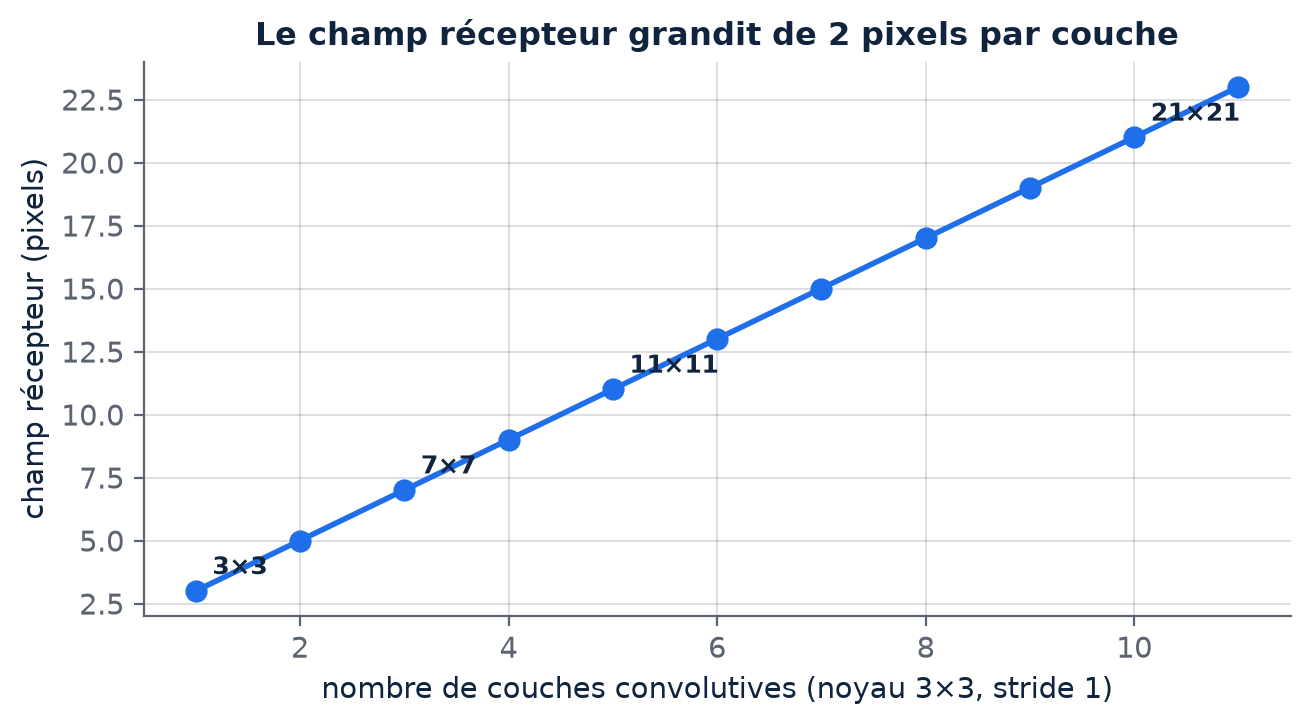
\includegraphics[width=.92\textwidth]{g09_champ_recepteur.png}\end{center}\end{frame}

\begin{frame}{Activité 2 --- suivre les dimensions d'une architecture}
\begin{abox}[À vous de jouer (15 min)]
Complétez le tableau : entrée $32 \times 32 \times 1$.
\begin{center}
\small
\begin{tabular}{@{}llll@{}}
\toprule
\textbf{Couche} & \textbf{Réglages} & \textbf{Sortie ?} & \\
\midrule
conv $5 \times 5$, 6 filtres & valid ($P=0$), $S=1$ & $?$ & \\
pool $2 \times 2$ & stride 2 & $?$ & \\
conv $5 \times 5$, 16 filtres & valid, $S=1$ & $?$ & \\
pool $2 \times 2$ & stride 2 & $?$ & \\
\bottomrule
\end{tabular}
\end{center}
\end{abox}
\begin{solbox}[Correction --- c'est l'architecture LeNet-5]

\end{solbox}
% [fix] bloc deplace
\end{frame}
\begin{frame}{Activité 2 --- suivre les dimensions d'u… (suite)}
\begin{center}
\small
\begin{tabular}{@{}lll@{}}
\toprule
\textbf{Couche} & \textbf{Calcul} & \textbf{Sortie} \\
\midrule
conv $5 \times 5$, 6 & $32 - 5 + 1$ & $28 \times 28 \times 6$ \\
pool $2 \times 2$ & $28 / 2$ & $14 \times 14 \times 6$ \\
conv $5 \times 5$, 16 & $14 - 5 + 1$ & $10 \times 10 \times 16$ \\
pool $2 \times 2$ & $10 / 2$ & $5 \times 5 \times 16$ \\
\bottomrule
\end{tabular}
\end{center}
\end{frame}

\begin{frame}{Quiz 3 --- padding, stride, dimensions}
\begin{qbox}[Question 1]
Entrée $11 \times 11$, noyau $3 \times 3$, padding $1$, stride $1$. Sortie ?
\begin{itemize}
  \item[(a)] $9 \times 9$ \quad (b) $11 \times 11$ \quad (c) $13 \times 13$
\end{itemize}
\end{qbox}
\begin{qbox}[Question 2]
Entrée $16 \times 16$, noyau $3 \times 3$, padding $0$, stride $2$. Sortie ?
\begin{itemize}
  \item[(a)] $8 \times 8$ \quad (b) $7 \times 7$ \quad (c) $14 \times 14$
\end{itemize}
\end{qbox}
\begin{qbox}[Question 3]
Trois couches convolutives $3 \times 3$ enchaînées (valid) équivalent, en champ
récepteur, à un noyau de côté :
\begin{itemize}
  \item[(a)] 6 \quad (b) 7 \quad (c) 9
\end{itemize}
\end{qbox}
\begin{solbox}[Réponses]
\textbf{1.} (b) : $(11 - 3 + 2)/1 + 1 = 11$. \quad
\textbf{2.} (b) : $(16 - 3)/2 + 1 = 7$ (partie entière de $6{,}5$). \quad
\textbf{3.} (b) : $1 + 2 \times 3 = 7$, donc $7 \times 7$.
\end{solbox}
\end{frame}
